% Created by tikzDevice version 0.12.6 on 2025-02-12 13:11:10
% !TEX encoding = UTF-8 Unicode
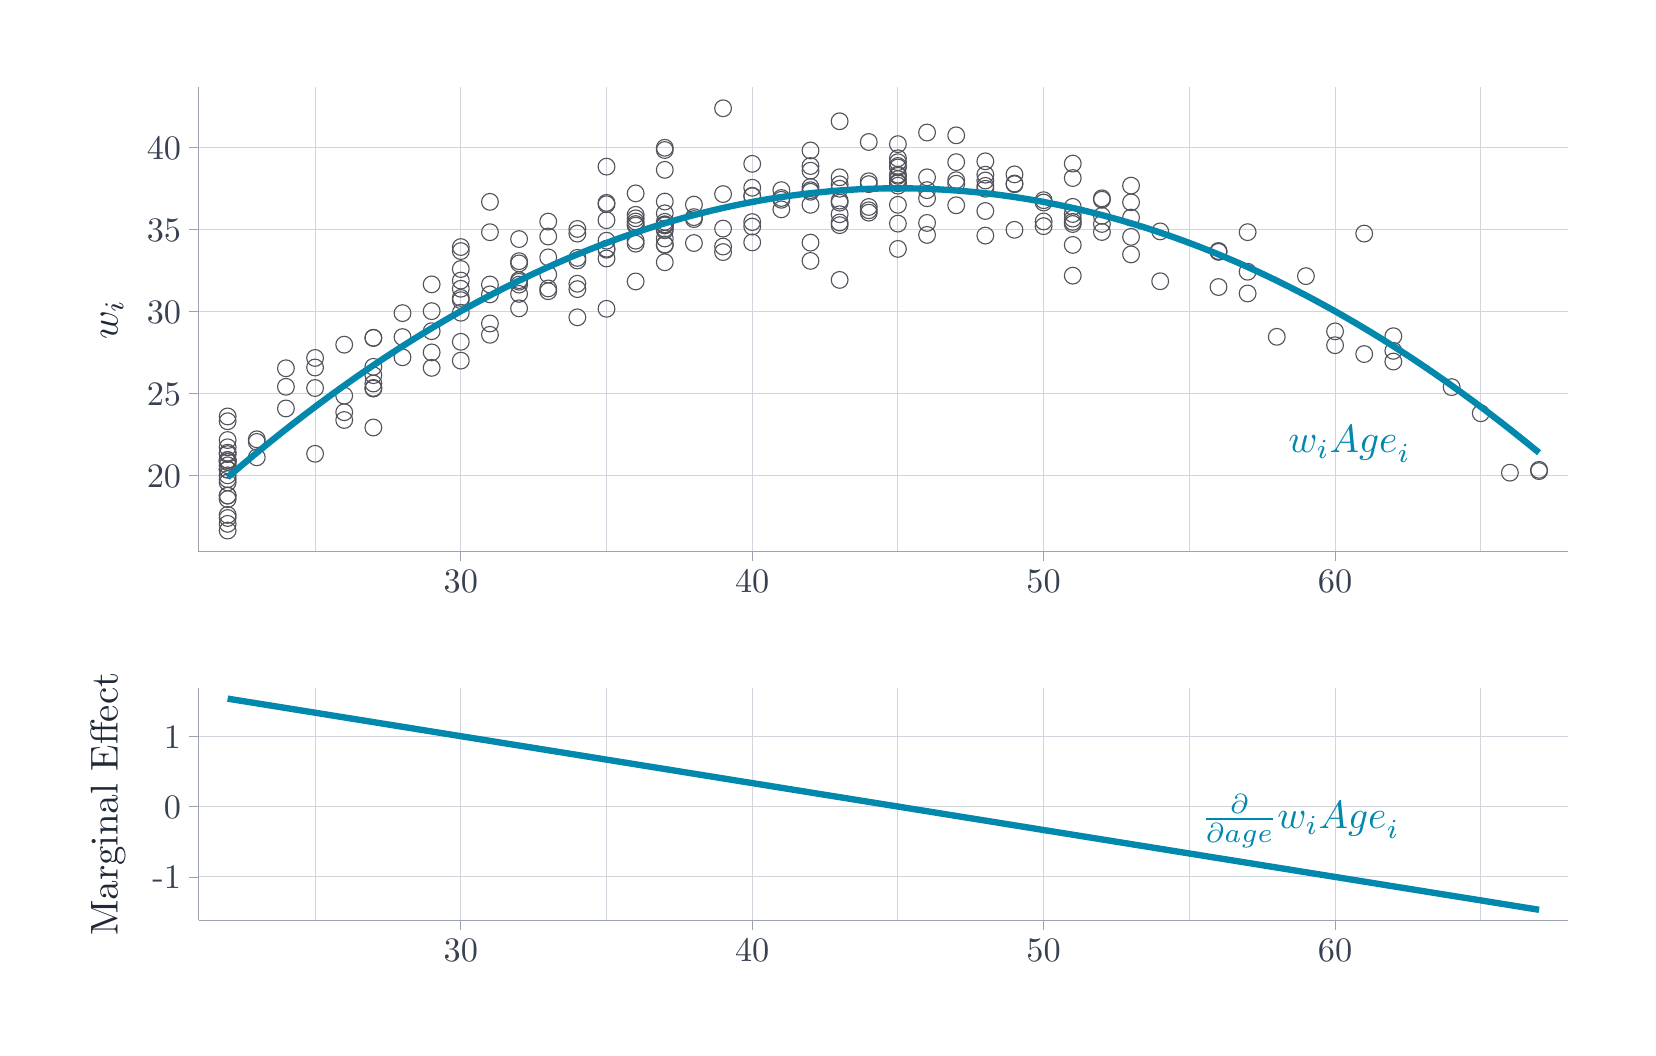
\begin{tikzpicture}[x=1pt,y=1pt]
\definecolor{fillColor}{RGB}{255,255,255}
\path[use as bounding box,fill=fillColor] (0,0) rectangle (578.16,361.35);
\begin{scope}
\path[clip] (  0.00,  0.00) rectangle (578.16,361.35);
\definecolor{drawColor}{RGB}{255,255,255}

\path[draw=drawColor,line width= 0.6pt,line join=round,line cap=round,fill=fillColor] (  0.00, -0.00) rectangle (578.16,361.35);
\end{scope}
\begin{scope}
\path[clip] (  5.50,138.71) rectangle (572.66,355.85);
\definecolor{drawColor}{RGB}{255,255,255}
\definecolor{fillColor}{RGB}{255,255,255}

\path[draw=drawColor,line width= 0.7pt,line join=round,line cap=round,fill=fillColor] (  5.50,138.71) rectangle (572.66,355.85);
\end{scope}
\begin{scope}
\path[clip] (  5.50,  5.50) rectangle (572.66,138.71);
\definecolor{drawColor}{RGB}{255,255,255}
\definecolor{fillColor}{RGB}{255,255,255}

\path[draw=drawColor,line width= 0.7pt,line join=round,line cap=round,fill=fillColor] (  5.50,  5.50) rectangle (572.66,138.71);
\end{scope}
\begin{scope}
\path[clip] ( 61.73,172.00) rectangle (556.66,339.85);
\definecolor{drawColor}{RGB}{255,255,255}
\definecolor{fillColor}{RGB}{255,255,255}

\path[draw=drawColor,line width= 0.7pt,line join=round,line cap=round,fill=fillColor] ( 61.73,172.00) rectangle (556.66,339.85);
\definecolor{drawColor}{RGB}{209,213,219}

\path[draw=drawColor,line width= 0.4pt,line join=round] (103.85,172.00) --
	(103.85,339.85);

\path[draw=drawColor,line width= 0.4pt,line join=round] (209.16,172.00) --
	(209.16,339.85);

\path[draw=drawColor,line width= 0.4pt,line join=round] (314.46,172.00) --
	(314.46,339.85);

\path[draw=drawColor,line width= 0.4pt,line join=round] (419.77,172.00) --
	(419.77,339.85);

\path[draw=drawColor,line width= 0.4pt,line join=round] (525.07,172.00) --
	(525.07,339.85);

\path[draw=drawColor,line width= 0.4pt,line join=round] ( 61.73,199.66) --
	(556.66,199.66);

\path[draw=drawColor,line width= 0.4pt,line join=round] ( 61.73,229.27) --
	(556.66,229.27);

\path[draw=drawColor,line width= 0.4pt,line join=round] ( 61.73,258.89) --
	(556.66,258.89);

\path[draw=drawColor,line width= 0.4pt,line join=round] ( 61.73,288.50) --
	(556.66,288.50);

\path[draw=drawColor,line width= 0.4pt,line join=round] ( 61.73,318.12) --
	(556.66,318.12);

\path[draw=drawColor,line width= 0.4pt,line join=round] (156.51,172.00) --
	(156.51,339.85);

\path[draw=drawColor,line width= 0.4pt,line join=round] (261.81,172.00) --
	(261.81,339.85);

\path[draw=drawColor,line width= 0.4pt,line join=round] (367.11,172.00) --
	(367.11,339.85);

\path[draw=drawColor,line width= 0.4pt,line join=round] (472.42,172.00) --
	(472.42,339.85);
\definecolor{drawColor}{RGB}{82,82,91}

\path[draw=drawColor,line width= 0.4pt,line join=round,line cap=round] (188.10,266.12) circle (  3.03);

\path[draw=drawColor,line width= 0.4pt,line join=round,line cap=round] (103.85,242.00) circle (  3.03);

\path[draw=drawColor,line width= 0.4pt,line join=round,line cap=round] (230.22,283.02) circle (  3.03);

\path[draw=drawColor,line width= 0.4pt,line join=round,line cap=round] (230.22,298.52) circle (  3.03);

\path[draw=drawColor,line width= 0.4pt,line join=round,line cap=round] (188.10,272.15) circle (  3.03);

\path[draw=drawColor,line width= 0.4pt,line join=round,line cap=round] (314.46,310.83) circle (  3.03);

\path[draw=drawColor,line width= 0.4pt,line join=round,line cap=round] (293.40,298.12) circle (  3.03);

\path[draw=drawColor,line width= 0.4pt,line join=round,line cap=round] (167.04,268.53) circle (  3.03);

\path[draw=drawColor,line width= 0.4pt,line join=round,line cap=round] ( 72.26,192.28) circle (  3.03);

\path[draw=drawColor,line width= 0.4pt,line join=round,line cap=round] (335.52,304.95) circle (  3.03);

\path[draw=drawColor,line width= 0.4pt,line join=round,line cap=round] (156.51,263.69) circle (  3.03);

\path[draw=drawColor,line width= 0.4pt,line join=round,line cap=round] (293.40,290.95) circle (  3.03);

\path[draw=drawColor,line width= 0.4pt,line join=round,line cap=round] (335.52,322.45) circle (  3.03);

\path[draw=drawColor,line width= 0.4pt,line join=round,line cap=round] (493.48,240.70) circle (  3.03);

\path[draw=drawColor,line width= 0.4pt,line join=round,line cap=round] ( 72.26,212.34) circle (  3.03);

\path[draw=drawColor,line width= 0.4pt,line join=round,line cap=round] (156.51,241.03) circle (  3.03);

\path[draw=drawColor,line width= 0.4pt,line join=round,line cap=round] (430.30,267.63) circle (  3.03);

\path[draw=drawColor,line width= 0.4pt,line join=round,line cap=round] (398.70,304.27) circle (  3.03);

\path[draw=drawColor,line width= 0.4pt,line join=round,line cap=round] (209.16,281.47) circle (  3.03);

\path[draw=drawColor,line width= 0.4pt,line join=round,line cap=round] (114.38,246.80) circle (  3.03);

\path[draw=drawColor,line width= 0.4pt,line join=round,line cap=round] (188.10,278.34) circle (  3.03);

\path[draw=drawColor,line width= 0.4pt,line join=round,line cap=round] ( 72.26,190.99) circle (  3.03);

\path[draw=drawColor,line width= 0.4pt,line join=round,line cap=round] (156.51,280.62) circle (  3.03);

\path[draw=drawColor,line width= 0.4pt,line join=round,line cap=round] (388.17,293.35) circle (  3.03);

\path[draw=drawColor,line width= 0.4pt,line join=round,line cap=round] (282.87,302.05) circle (  3.03);

\path[draw=drawColor,line width= 0.4pt,line join=round,line cap=round] (335.52,312.75) circle (  3.03);

\path[draw=drawColor,line width= 0.4pt,line join=round,line cap=round] (377.64,271.73) circle (  3.03);

\path[draw=drawColor,line width= 0.4pt,line join=round,line cap=round] (230.22,288.72) circle (  3.03);

\path[draw=drawColor,line width= 0.4pt,line join=round,line cap=round] ( 72.26,209.72) circle (  3.03);

\path[draw=drawColor,line width= 0.4pt,line join=round,line cap=round] (240.75,283.53) circle (  3.03);

\path[draw=drawColor,line width= 0.4pt,line join=round,line cap=round] (314.46,306.64) circle (  3.03);

\path[draw=drawColor,line width= 0.4pt,line join=round,line cap=round] ( 93.32,238.27) circle (  3.03);

\path[draw=drawColor,line width= 0.4pt,line join=round,line cap=round] (367.11,289.62) circle (  3.03);

\path[draw=drawColor,line width= 0.4pt,line join=round,line cap=round] (230.22,290.12) circle (  3.03);

\path[draw=drawColor,line width= 0.4pt,line join=round,line cap=round] (293.40,293.93) circle (  3.03);

\path[draw=drawColor,line width= 0.4pt,line join=round,line cap=round] (398.70,298.25) circle (  3.03);

\path[draw=drawColor,line width= 0.4pt,line join=round,line cap=round] (546.13,201.57) circle (  3.03);

\path[draw=drawColor,line width= 0.4pt,line join=round,line cap=round] (209.16,281.11) circle (  3.03);

\path[draw=drawColor,line width= 0.4pt,line join=round,line cap=round] (219.69,289.82) circle (  3.03);

\path[draw=drawColor,line width= 0.4pt,line join=round,line cap=round] (377.64,296.59) circle (  3.03);

\path[draw=drawColor,line width= 0.4pt,line join=round,line cap=round] (219.69,301.47) circle (  3.03);

\path[draw=drawColor,line width= 0.4pt,line join=round,line cap=round] (230.22,276.58) circle (  3.03);

\path[draw=drawColor,line width= 0.4pt,line join=round,line cap=round] (114.38,228.37) circle (  3.03);

\path[draw=drawColor,line width= 0.4pt,line join=round,line cap=round] (230.22,289.88) circle (  3.03);

\path[draw=drawColor,line width= 0.4pt,line join=round,line cap=round] (314.46,312.74) circle (  3.03);

\path[draw=drawColor,line width= 0.4pt,line join=round,line cap=round] (114.38,219.58) circle (  3.03);

\path[draw=drawColor,line width= 0.4pt,line join=round,line cap=round] (430.30,280.44) circle (  3.03);

\path[draw=drawColor,line width= 0.4pt,line join=round,line cap=round] (167.04,264.97) circle (  3.03);

\path[draw=drawColor,line width= 0.4pt,line join=round,line cap=round] ( 72.26,201.61) circle (  3.03);

\path[draw=drawColor,line width= 0.4pt,line join=round,line cap=round] (240.75,297.41) circle (  3.03);

\path[draw=drawColor,line width= 0.4pt,line join=round,line cap=round] (219.69,290.39) circle (  3.03);

\path[draw=drawColor,line width= 0.4pt,line join=round,line cap=round] (198.63,268.82) circle (  3.03);

\path[draw=drawColor,line width= 0.4pt,line join=round,line cap=round] (482.95,243.41) circle (  3.03);

\path[draw=drawColor,line width= 0.4pt,line join=round,line cap=round] (388.17,290.42) circle (  3.03);

\path[draw=drawColor,line width= 0.4pt,line join=round,line cap=round] (282.87,316.97) circle (  3.03);

\path[draw=drawColor,line width= 0.4pt,line join=round,line cap=round] ( 82.79,212.61) circle (  3.03);

\path[draw=drawColor,line width= 0.4pt,line join=round,line cap=round] ( 72.26,182.06) circle (  3.03);

\path[draw=drawColor,line width= 0.4pt,line join=round,line cap=round] (388.17,299.17) circle (  3.03);

\path[draw=drawColor,line width= 0.4pt,line join=round,line cap=round] (219.69,291.30) circle (  3.03);

\path[draw=drawColor,line width= 0.4pt,line join=round,line cap=round] (314.46,319.26) circle (  3.03);

\path[draw=drawColor,line width= 0.4pt,line join=round,line cap=round] ( 72.26,220.87) circle (  3.03);

\path[draw=drawColor,line width= 0.4pt,line join=round,line cap=round] (535.60,200.54) circle (  3.03);

\path[draw=drawColor,line width= 0.4pt,line join=round,line cap=round] (303.93,294.50) circle (  3.03);

\path[draw=drawColor,line width= 0.4pt,line join=round,line cap=round] (314.46,305.12) circle (  3.03);

\path[draw=drawColor,line width= 0.4pt,line join=round,line cap=round] (156.51,269.96) circle (  3.03);

\path[draw=drawColor,line width= 0.4pt,line join=round,line cap=round] (261.81,303.51) circle (  3.03);

\path[draw=drawColor,line width= 0.4pt,line join=round,line cap=round] (282.87,277.07) circle (  3.03);

\path[draw=drawColor,line width= 0.4pt,line join=round,line cap=round] (198.63,256.68) circle (  3.03);

\path[draw=drawColor,line width= 0.4pt,line join=round,line cap=round] (156.51,247.84) circle (  3.03);

\path[draw=drawColor,line width= 0.4pt,line join=round,line cap=round] (230.22,288.13) circle (  3.03);

\path[draw=drawColor,line width= 0.4pt,line join=round,line cap=round] (346.05,308.22) circle (  3.03);

\path[draw=drawColor,line width= 0.4pt,line join=round,line cap=round] (440.83,273.15) circle (  3.03);

\path[draw=drawColor,line width= 0.4pt,line join=round,line cap=round] ( 72.26,203.21) circle (  3.03);

\path[draw=drawColor,line width= 0.4pt,line join=round,line cap=round] (356.58,308.33) circle (  3.03);

\path[draw=drawColor,line width= 0.4pt,line join=round,line cap=round] ( 72.26,179.63) circle (  3.03);

\path[draw=drawColor,line width= 0.4pt,line join=round,line cap=round] (230.22,290.31) circle (  3.03);

\path[draw=drawColor,line width= 0.4pt,line join=round,line cap=round] (188.10,267.12) circle (  3.03);

\path[draw=drawColor,line width= 0.4pt,line join=round,line cap=round] (356.58,304.78) circle (  3.03);

\path[draw=drawColor,line width= 0.4pt,line join=round,line cap=round] (156.51,267.01) circle (  3.03);

\path[draw=drawColor,line width= 0.4pt,line join=round,line cap=round] ( 82.79,206.10) circle (  3.03);

\path[draw=drawColor,line width= 0.4pt,line join=round,line cap=round] (124.91,238.79) circle (  3.03);

\path[draw=drawColor,line width= 0.4pt,line join=round,line cap=round] (261.81,300.61) circle (  3.03);

\path[draw=drawColor,line width= 0.4pt,line join=round,line cap=round] (124.91,230.93) circle (  3.03);

\path[draw=drawColor,line width= 0.4pt,line join=round,line cap=round] (314.46,281.40) circle (  3.03);

\path[draw=drawColor,line width= 0.4pt,line join=round,line cap=round] (388.17,287.52) circle (  3.03);

\path[draw=drawColor,line width= 0.4pt,line join=round,line cap=round] (124.91,249.21) circle (  3.03);

\path[draw=drawColor,line width= 0.4pt,line join=round,line cap=round] (346.05,303.13) circle (  3.03);

\path[draw=drawColor,line width= 0.4pt,line join=round,line cap=round] (293.40,307.28) circle (  3.03);

\path[draw=drawColor,line width= 0.4pt,line join=round,line cap=round] (303.93,296.55) circle (  3.03);

\path[draw=drawColor,line width= 0.4pt,line join=round,line cap=round] (367.11,299.01) circle (  3.03);

\path[draw=drawColor,line width= 0.4pt,line join=round,line cap=round] (198.63,288.62) circle (  3.03);

\path[draw=drawColor,line width= 0.4pt,line join=round,line cap=round] (314.46,304.25) circle (  3.03);

\path[draw=drawColor,line width= 0.4pt,line join=round,line cap=round] (451.36,249.64) circle (  3.03);

\path[draw=drawColor,line width= 0.4pt,line join=round,line cap=round] (482.95,286.94) circle (  3.03);

\path[draw=drawColor,line width= 0.4pt,line join=round,line cap=round] (398.70,285.76) circle (  3.03);

\path[draw=drawColor,line width= 0.4pt,line join=round,line cap=round] (177.57,259.92) circle (  3.03);

\path[draw=drawColor,line width= 0.4pt,line join=round,line cap=round] (346.05,313.06) circle (  3.03);

\path[draw=drawColor,line width= 0.4pt,line join=round,line cap=round] (314.46,311.38) circle (  3.03);

\path[draw=drawColor,line width= 0.4pt,line join=round,line cap=round] ( 72.26,205.15) circle (  3.03);

\path[draw=drawColor,line width= 0.4pt,line join=round,line cap=round] ( 72.26,198.20) circle (  3.03);

\path[draw=drawColor,line width= 0.4pt,line join=round,line cap=round] (398.70,292.73) circle (  3.03);

\path[draw=drawColor,line width= 0.4pt,line join=round,line cap=round] (219.69,293.72) circle (  3.03);

\path[draw=drawColor,line width= 0.4pt,line join=round,line cap=round] (219.69,292.46) circle (  3.03);

\path[draw=drawColor,line width= 0.4pt,line join=round,line cap=round] (219.69,269.65) circle (  3.03);

\path[draw=drawColor,line width= 0.4pt,line join=round,line cap=round] ( 72.26,204.44) circle (  3.03);

\path[draw=drawColor,line width= 0.4pt,line join=round,line cap=round] (377.64,307.01) circle (  3.03);

\path[draw=drawColor,line width= 0.4pt,line join=round,line cap=round] (261.81,312.14) circle (  3.03);

\path[draw=drawColor,line width= 0.4pt,line join=round,line cap=round] (314.46,297.34) circle (  3.03);

\path[draw=drawColor,line width= 0.4pt,line join=round,line cap=round] (261.81,300.44) circle (  3.03);

\path[draw=drawColor,line width= 0.4pt,line join=round,line cap=round] ( 93.32,223.75) circle (  3.03);

\path[draw=drawColor,line width= 0.4pt,line join=round,line cap=round] (324.99,302.64) circle (  3.03);

\path[draw=drawColor,line width= 0.4pt,line join=round,line cap=round] (114.38,222.39) circle (  3.03);

\path[draw=drawColor,line width= 0.4pt,line join=round,line cap=round] (230.22,291.18) circle (  3.03);

\path[draw=drawColor,line width= 0.4pt,line join=round,line cap=round] (346.05,295.10) circle (  3.03);

\path[draw=drawColor,line width= 0.4pt,line join=round,line cap=round] (346.05,286.22) circle (  3.03);

\path[draw=drawColor,line width= 0.4pt,line join=round,line cap=round] (335.52,297.17) circle (  3.03);

\path[draw=drawColor,line width= 0.4pt,line join=round,line cap=round] (156.51,258.34) circle (  3.03);

\path[draw=drawColor,line width= 0.4pt,line join=round,line cap=round] (167.04,287.44) circle (  3.03);

\path[draw=drawColor,line width= 0.4pt,line join=round,line cap=round] (177.57,268.51) circle (  3.03);

\path[draw=drawColor,line width= 0.4pt,line join=round,line cap=round] (198.63,266.86) circle (  3.03);

\path[draw=drawColor,line width= 0.4pt,line join=round,line cap=round] (145.98,238.42) circle (  3.03);

\path[draw=drawColor,line width= 0.4pt,line join=round,line cap=round] (272.34,302.64) circle (  3.03);

\path[draw=drawColor,line width= 0.4pt,line join=round,line cap=round] (209.16,284.37) circle (  3.03);

\path[draw=drawColor,line width= 0.4pt,line join=round,line cap=round] (356.58,305.03) circle (  3.03);

\path[draw=drawColor,line width= 0.4pt,line join=round,line cap=round] (251.28,280.26) circle (  3.03);

\path[draw=drawColor,line width= 0.4pt,line join=round,line cap=round] (377.64,290.40) circle (  3.03);

\path[draw=drawColor,line width= 0.4pt,line join=round,line cap=round] (209.16,291.78) circle (  3.03);

\path[draw=drawColor,line width= 0.4pt,line join=round,line cap=round] (251.28,301.22) circle (  3.03);

\path[draw=drawColor,line width= 0.4pt,line join=round,line cap=round] (209.16,259.76) circle (  3.03);

\path[draw=drawColor,line width= 0.4pt,line join=round,line cap=round] (303.93,305.85) circle (  3.03);

\path[draw=drawColor,line width= 0.4pt,line join=round,line cap=round] (377.64,291.17) circle (  3.03);

\path[draw=drawColor,line width= 0.4pt,line join=round,line cap=round] (209.16,298.04) circle (  3.03);

\path[draw=drawColor,line width= 0.4pt,line join=round,line cap=round] (124.91,235.78) circle (  3.03);

\path[draw=drawColor,line width= 0.4pt,line join=round,line cap=round] (198.63,286.93) circle (  3.03);

\path[draw=drawColor,line width= 0.4pt,line join=round,line cap=round] (124.91,249.30) circle (  3.03);

\path[draw=drawColor,line width= 0.4pt,line join=round,line cap=round] (251.28,332.22) circle (  3.03);

\path[draw=drawColor,line width= 0.4pt,line join=round,line cap=round] (409.23,269.72) circle (  3.03);

\path[draw=drawColor,line width= 0.4pt,line join=round,line cap=round] (282.87,311.35) circle (  3.03);

\path[draw=drawColor,line width= 0.4pt,line join=round,line cap=round] (461.89,271.57) circle (  3.03);

\path[draw=drawColor,line width= 0.4pt,line join=round,line cap=round] (346.05,306.12) circle (  3.03);

\path[draw=drawColor,line width= 0.4pt,line join=round,line cap=round] (282.87,309.66) circle (  3.03);

\path[draw=drawColor,line width= 0.4pt,line join=round,line cap=round] (251.28,282.26) circle (  3.03);

\path[draw=drawColor,line width= 0.4pt,line join=round,line cap=round] (219.69,284.37) circle (  3.03);

\path[draw=drawColor,line width= 0.4pt,line join=round,line cap=round] (356.58,288.30) circle (  3.03);

\path[draw=drawColor,line width= 0.4pt,line join=round,line cap=round] (198.63,278.16) circle (  3.03);

\path[draw=drawColor,line width= 0.4pt,line join=round,line cap=round] ( 72.26,219.13) circle (  3.03);

\path[draw=drawColor,line width= 0.4pt,line join=round,line cap=round] (493.48,249.86) circle (  3.03);

\path[draw=drawColor,line width= 0.4pt,line join=round,line cap=round] (324.99,290.79) circle (  3.03);

\path[draw=drawColor,line width= 0.4pt,line join=round,line cap=round] (209.16,311.13) circle (  3.03);

\path[draw=drawColor,line width= 0.4pt,line join=round,line cap=round] (293.40,289.99) circle (  3.03);

\path[draw=drawColor,line width= 0.4pt,line join=round,line cap=round] (124.91,231.18) circle (  3.03);

\path[draw=drawColor,line width= 0.4pt,line join=round,line cap=round] (209.16,297.54) circle (  3.03);

\path[draw=drawColor,line width= 0.4pt,line join=round,line cap=round] (240.75,292.88) circle (  3.03);

\path[draw=drawColor,line width= 0.4pt,line join=round,line cap=round] (135.45,249.54) circle (  3.03);

\path[draw=drawColor,line width= 0.4pt,line join=round,line cap=round] ( 72.26,185.27) circle (  3.03);

\path[draw=drawColor,line width= 0.4pt,line join=round,line cap=round] (272.34,299.80) circle (  3.03);

\path[draw=drawColor,line width= 0.4pt,line join=round,line cap=round] (293.40,303.15) circle (  3.03);

\path[draw=drawColor,line width= 0.4pt,line join=round,line cap=round] (261.81,283.76) circle (  3.03);

\path[draw=drawColor,line width= 0.4pt,line join=round,line cap=round] (314.46,314.15) circle (  3.03);

\path[draw=drawColor,line width= 0.4pt,line join=round,line cap=round] (440.83,265.30) circle (  3.03);

\path[draw=drawColor,line width= 0.4pt,line join=round,line cap=round] (124.91,232.77) circle (  3.03);

\path[draw=drawColor,line width= 0.4pt,line join=round,line cap=round] (209.16,277.95) circle (  3.03);

\path[draw=drawColor,line width= 0.4pt,line join=round,line cap=round] (472.42,246.60) circle (  3.03);

\path[draw=drawColor,line width= 0.4pt,line join=round,line cap=round] (230.22,294.26) circle (  3.03);

\path[draw=drawColor,line width= 0.4pt,line join=round,line cap=round] ( 93.32,231.58) circle (  3.03);

\path[draw=drawColor,line width= 0.4pt,line join=round,line cap=round] (303.93,320.04) circle (  3.03);

\path[draw=drawColor,line width= 0.4pt,line join=round,line cap=round] (272.34,299.15) circle (  3.03);

\path[draw=drawColor,line width= 0.4pt,line join=round,line cap=round] (324.99,323.46) circle (  3.03);

\path[draw=drawColor,line width= 0.4pt,line join=round,line cap=round] (388.17,299.68) circle (  3.03);

\path[draw=drawColor,line width= 0.4pt,line join=round,line cap=round] (188.10,285.88) circle (  3.03);

\path[draw=drawColor,line width= 0.4pt,line join=round,line cap=round] (198.63,277.21) circle (  3.03);

\path[draw=drawColor,line width= 0.4pt,line join=round,line cap=round] (135.45,242.25) circle (  3.03);

\path[draw=drawColor,line width= 0.4pt,line join=round,line cap=round] ( 72.26,204.43) circle (  3.03);

\path[draw=drawColor,line width= 0.4pt,line join=round,line cap=round] (177.57,276.97) circle (  3.03);

\path[draw=drawColor,line width= 0.4pt,line join=round,line cap=round] ( 72.26,201.67) circle (  3.03);

\path[draw=drawColor,line width= 0.4pt,line join=round,line cap=round] (282.87,302.62) circle (  3.03);

\path[draw=drawColor,line width= 0.4pt,line join=round,line cap=round] (103.85,238.55) circle (  3.03);

\path[draw=drawColor,line width= 0.4pt,line join=round,line cap=round] (156.51,282.07) circle (  3.03);

\path[draw=drawColor,line width= 0.4pt,line join=round,line cap=round] (240.75,292.18) circle (  3.03);

\path[draw=drawColor,line width= 0.4pt,line join=round,line cap=round] ( 72.26,197.00) circle (  3.03);

\path[draw=drawColor,line width= 0.4pt,line join=round,line cap=round] (177.57,269.54) circle (  3.03);

\path[draw=drawColor,line width= 0.4pt,line join=round,line cap=round] (230.22,309.97) circle (  3.03);

\path[draw=drawColor,line width= 0.4pt,line join=round,line cap=round] (230.22,317.14) circle (  3.03);

\path[draw=drawColor,line width= 0.4pt,line join=round,line cap=round] (346.05,304.18) circle (  3.03);

\path[draw=drawColor,line width= 0.4pt,line join=round,line cap=round] (367.11,291.33) circle (  3.03);

\path[draw=drawColor,line width= 0.4pt,line join=round,line cap=round] (546.13,201.12) circle (  3.03);

\path[draw=drawColor,line width= 0.4pt,line join=round,line cap=round] (177.57,265.15) circle (  3.03);

\path[draw=drawColor,line width= 0.4pt,line join=round,line cap=round] (272.34,295.70) circle (  3.03);

\path[draw=drawColor,line width= 0.4pt,line join=round,line cap=round] (156.51,262.88) circle (  3.03);

\path[draw=drawColor,line width= 0.4pt,line join=round,line cap=round] (282.87,303.78) circle (  3.03);

\path[draw=drawColor,line width= 0.4pt,line join=round,line cap=round] (377.64,312.24) circle (  3.03);

\path[draw=drawColor,line width= 0.4pt,line join=round,line cap=round] (324.99,299.70) circle (  3.03);

\path[draw=drawColor,line width= 0.4pt,line join=round,line cap=round] (177.57,284.96) circle (  3.03);

\path[draw=drawColor,line width= 0.4pt,line join=round,line cap=round] (377.64,292.36) circle (  3.03);

\path[draw=drawColor,line width= 0.4pt,line join=round,line cap=round] (282.87,283.67) circle (  3.03);

\path[draw=drawColor,line width= 0.4pt,line join=round,line cap=round] ( 72.26,199.59) circle (  3.03);

\path[draw=drawColor,line width= 0.4pt,line join=round,line cap=round] (167.04,250.37) circle (  3.03);

\path[draw=drawColor,line width= 0.4pt,line join=round,line cap=round] (377.64,294.02) circle (  3.03);

\path[draw=drawColor,line width= 0.4pt,line join=round,line cap=round] (251.28,288.74) circle (  3.03);

\path[draw=drawColor,line width= 0.4pt,line join=round,line cap=round] (377.64,282.84) circle (  3.03);

\path[draw=drawColor,line width= 0.4pt,line join=round,line cap=round] (324.99,286.46) circle (  3.03);

\path[draw=drawColor,line width= 0.4pt,line join=round,line cap=round] ( 82.79,211.66) circle (  3.03);

\path[draw=drawColor,line width= 0.4pt,line join=round,line cap=round] (409.23,287.73) circle (  3.03);

\path[draw=drawColor,line width= 0.4pt,line join=round,line cap=round] (430.30,280.64) circle (  3.03);

\path[draw=drawColor,line width= 0.4pt,line join=round,line cap=round] (430.30,280.34) circle (  3.03);

\path[draw=drawColor,line width= 0.4pt,line join=round,line cap=round] (230.22,317.95) circle (  3.03);

\path[draw=drawColor,line width= 0.4pt,line join=round,line cap=round] (303.93,295.37) circle (  3.03);

\path[draw=drawColor,line width= 0.4pt,line join=round,line cap=round] (230.22,285.16) circle (  3.03);

\path[draw=drawColor,line width= 0.4pt,line join=round,line cap=round] (156.51,274.14) circle (  3.03);

\path[draw=drawColor,line width= 0.4pt,line join=round,line cap=round] (314.46,290.54) circle (  3.03);

\path[draw=drawColor,line width= 0.4pt,line join=round,line cap=round] (525.07,222.01) circle (  3.03);

\path[draw=drawColor,line width= 0.4pt,line join=round,line cap=round] (293.40,304.74) circle (  3.03);

\path[draw=drawColor,line width= 0.4pt,line join=round,line cap=round] ( 72.26,207.77) circle (  3.03);

\path[draw=drawColor,line width= 0.4pt,line join=round,line cap=round] ( 72.26,205.08) circle (  3.03);

\path[draw=drawColor,line width= 0.4pt,line join=round,line cap=round] (230.22,282.81) circle (  3.03);

\path[draw=drawColor,line width= 0.4pt,line join=round,line cap=round] (293.40,298.86) circle (  3.03);

\path[draw=drawColor,line width= 0.4pt,line join=round,line cap=round] (167.04,254.45) circle (  3.03);

\path[draw=drawColor,line width= 0.4pt,line join=round,line cap=round] (440.83,287.45) circle (  3.03);

\path[draw=drawColor,line width= 0.4pt,line join=round,line cap=round] ( 72.26,207.26) circle (  3.03);

\path[draw=drawColor,line width= 0.4pt,line join=round,line cap=round] (124.91,216.87) circle (  3.03);

\path[draw=drawColor,line width= 0.4pt,line join=round,line cap=round] (103.85,231.14) circle (  3.03);

\path[draw=drawColor,line width= 0.4pt,line join=round,line cap=round] (261.81,289.47) circle (  3.03);

\path[draw=drawColor,line width= 0.4pt,line join=round,line cap=round] (472.42,251.61) circle (  3.03);

\path[draw=drawColor,line width= 0.4pt,line join=round,line cap=round] (177.57,276.16) circle (  3.03);

\path[draw=drawColor,line width= 0.4pt,line join=round,line cap=round] (335.52,306.23) circle (  3.03);

\path[draw=drawColor,line width= 0.4pt,line join=round,line cap=round] (314.46,308.24) circle (  3.03);

\path[draw=drawColor,line width= 0.4pt,line join=round,line cap=round] (303.93,304.81) circle (  3.03);

\path[draw=drawColor,line width= 0.4pt,line join=round,line cap=round] (188.10,291.27) circle (  3.03);

\path[draw=drawColor,line width= 0.4pt,line join=round,line cap=round] (293.40,327.53) circle (  3.03);

\path[draw=drawColor,line width= 0.4pt,line join=round,line cap=round] (261.81,291.10) circle (  3.03);

\path[draw=drawColor,line width= 0.4pt,line join=round,line cap=round] (493.48,244.57) circle (  3.03);

\path[draw=drawColor,line width= 0.4pt,line join=round,line cap=round] (514.54,231.46) circle (  3.03);

\path[draw=drawColor,line width= 0.4pt,line join=round,line cap=round] (293.40,270.20) circle (  3.03);

\path[draw=drawColor,line width= 0.4pt,line join=round,line cap=round] ( 72.26,184.17) circle (  3.03);

\path[draw=drawColor,line width= 0.4pt,line join=round,line cap=round] (219.69,283.29) circle (  3.03);

\path[draw=drawColor,line width= 0.4pt,line join=round,line cap=round] (314.46,305.43) circle (  3.03);

\path[draw=drawColor,line width= 0.4pt,line join=round,line cap=round] (367.11,298.17) circle (  3.03);

\path[draw=drawColor,line width= 0.4pt,line join=round,line cap=round] ( 72.26,192.26) circle (  3.03);

\path[draw=drawColor,line width= 0.4pt,line join=round,line cap=round] (135.45,258.20) circle (  3.03);

\path[draw=drawColor,line width= 0.4pt,line join=round,line cap=round] (167.04,298.41) circle (  3.03);

\path[draw=drawColor,line width= 0.4pt,line join=round,line cap=round] (282.87,297.34) circle (  3.03);

\path[draw=drawColor,line width= 0.4pt,line join=round,line cap=round] (145.98,268.59) circle (  3.03);

\path[draw=drawColor,line width= 0.4pt,line join=round,line cap=round] (103.85,207.37) circle (  3.03);

\path[draw=drawColor,line width= 0.4pt,line join=round,line cap=round] (398.70,279.41) circle (  3.03);

\path[draw=drawColor,line width= 0.4pt,line join=round,line cap=round] (145.98,251.67) circle (  3.03);

\path[draw=drawColor,line width= 0.4pt,line join=round,line cap=round] (314.46,307.81) circle (  3.03);

\path[draw=drawColor,line width= 0.4pt,line join=round,line cap=round] (324.99,307.27) circle (  3.03);

\path[draw=drawColor,line width= 0.4pt,line join=round,line cap=round] (145.98,244.01) circle (  3.03);

\path[draw=drawColor,line width= 0.4pt,line join=round,line cap=round] (177.57,270.12) circle (  3.03);

\path[draw=drawColor,line width= 0.4pt,line join=round,line cap=round] (145.98,258.91) circle (  3.03);
\definecolor{drawColor}{RGB}{1,136,172}

\path[draw=drawColor,line width= 2.3pt,line join=round] ( 72.26,198.87) --
	( 77.00,202.91) --
	( 81.74,206.88) --
	( 86.48,210.77) --
	( 91.22,214.58) --
	( 95.96,218.30) --
	(100.70,221.95) --
	(105.43,225.52) --
	(110.17,229.00) --
	(114.91,232.41) --
	(119.65,235.74) --
	(124.39,238.99) --
	(129.13,242.15) --
	(133.87,245.24) --
	(138.60,248.25) --
	(143.34,251.17) --
	(148.08,254.02) --
	(152.82,256.79) --
	(157.56,259.48) --
	(162.30,262.08) --
	(167.04,264.61) --
	(171.78,267.06) --
	(176.51,269.43) --
	(181.25,271.71) --
	(185.99,273.92) --
	(190.73,276.05) --
	(195.47,278.10) --
	(200.21,280.07) --
	(204.95,281.95) --
	(209.68,283.76) --
	(214.42,285.49) --
	(219.16,287.14) --
	(223.90,288.71) --
	(228.64,290.19) --
	(233.38,291.60) --
	(238.12,292.93) --
	(242.86,294.18) --
	(247.59,295.35) --
	(252.33,296.44) --
	(257.07,297.44) --
	(261.81,298.37) --
	(266.55,299.22) --
	(271.29,299.99) --
	(276.03,300.68) --
	(280.76,301.29) --
	(285.50,301.81) --
	(290.24,302.26) --
	(294.98,302.63) --
	(299.72,302.92) --
	(304.46,303.13) --
	(309.20,303.26) --
	(313.94,303.31) --
	(318.67,303.28) --
	(323.41,303.17) --
	(328.15,302.97) --
	(332.89,302.70) --
	(337.63,302.35) --
	(342.37,301.92) --
	(347.11,301.41) --
	(351.84,300.82) --
	(356.58,300.15) --
	(361.32,299.40) --
	(366.06,298.57) --
	(370.80,297.66) --
	(375.54,296.67) --
	(380.28,295.60) --
	(385.02,294.45) --
	(389.75,293.21) --
	(394.49,291.90) --
	(399.23,290.51) --
	(403.97,289.04) --
	(408.71,287.49) --
	(413.45,285.86) --
	(418.19,284.15) --
	(422.92,282.36) --
	(427.66,280.49) --
	(432.40,278.54) --
	(437.14,276.51) --
	(441.88,274.40) --
	(446.62,272.21) --
	(451.36,269.94) --
	(456.10,267.59) --
	(460.83,265.16) --
	(465.57,262.65) --
	(470.31,260.06) --
	(475.05,257.39) --
	(479.79,254.64) --
	(484.53,251.81) --
	(489.27,248.90) --
	(494.00,245.91) --
	(498.74,242.85) --
	(503.48,239.70) --
	(508.22,236.47) --
	(512.96,233.16) --
	(517.70,229.77) --
	(522.44,226.30) --
	(527.17,222.75) --
	(531.91,219.12) --
	(536.65,215.41) --
	(541.39,211.62) --
	(546.13,207.75);

\path[] (424.32,203.54) --
	(501.44,203.54) --
	(501.33,203.54) --
	(501.75,203.56) --
	(502.15,203.64) --
	(502.54,203.79) --
	(502.90,203.99) --
	(503.22,204.26) --
	(503.49,204.57) --
	(503.71,204.92) --
	(503.88,205.30) --
	(503.97,205.70) --
	(504.01,206.11) --
	(504.01,206.11) --
	(504.01,218.87) --
	(504.01,218.87) --
	(503.97,219.28) --
	(503.88,219.69) --
	(503.71,220.07) --
	(503.49,220.42) --
	(503.22,220.73) --
	(502.90,220.99) --
	(502.54,221.19) --
	(502.15,221.34) --
	(501.75,221.42) --
	(501.44,221.44) --
	(424.32,221.44) --
	(424.63,221.42) --
	(424.22,221.44) --
	(423.81,221.39) --
	(423.41,221.27) --
	(423.04,221.10) --
	(422.70,220.86) --
	(422.40,220.58) --
	(422.15,220.25) --
	(421.96,219.88) --
	(421.83,219.49) --
	(421.76,219.08) --
	(421.75,218.87) --
	(421.75,206.11) --
	(421.76,206.32) --
	(421.76,205.90) --
	(421.83,205.49) --
	(421.96,205.10) --
	(422.15,204.74) --
	(422.40,204.41) --
	(422.70,204.12) --
	(423.04,203.88) --
	(423.41,203.71) --
	(423.81,203.59) --
	(424.22,203.54) --
	cycle;
\end{scope}
\begin{scope}
\path[clip] ( 61.73,172.00) rectangle (556.66,339.85);
\definecolor{drawColor}{RGB}{1,136,172}

\node[text=drawColor,anchor=base east,inner sep=0pt, outer sep=0pt, scale=  1.42] at (499.72,207.82) {$\expec{w_i}{\text{Age}_i}$};
\end{scope}
\begin{scope}
\path[clip] (  0.00,  0.00) rectangle (578.16,361.35);
\definecolor{drawColor}{RGB}{156,163,175}

\path[draw=drawColor,line width= 0.3pt,line join=round] ( 61.73,172.00) --
	( 61.73,339.85);
\end{scope}
\begin{scope}
\path[clip] (  0.00,  0.00) rectangle (578.16,361.35);
\definecolor{drawColor}{RGB}{55,65,81}

\node[text=drawColor,anchor=base east,inner sep=0pt, outer sep=0pt, scale=  1.24] at ( 55.43,195.37) {20};

\node[text=drawColor,anchor=base east,inner sep=0pt, outer sep=0pt, scale=  1.24] at ( 55.43,224.99) {25};

\node[text=drawColor,anchor=base east,inner sep=0pt, outer sep=0pt, scale=  1.24] at ( 55.43,254.60) {30};

\node[text=drawColor,anchor=base east,inner sep=0pt, outer sep=0pt, scale=  1.24] at ( 55.43,284.22) {35};

\node[text=drawColor,anchor=base east,inner sep=0pt, outer sep=0pt, scale=  1.24] at ( 55.43,313.83) {40};
\end{scope}
\begin{scope}
\path[clip] (  0.00,  0.00) rectangle (578.16,361.35);
\definecolor{drawColor}{RGB}{156,163,175}

\path[draw=drawColor,line width= 0.3pt,line join=round] ( 58.23,199.66) --
	( 61.73,199.66);

\path[draw=drawColor,line width= 0.3pt,line join=round] ( 58.23,229.27) --
	( 61.73,229.27);

\path[draw=drawColor,line width= 0.3pt,line join=round] ( 58.23,258.89) --
	( 61.73,258.89);

\path[draw=drawColor,line width= 0.3pt,line join=round] ( 58.23,288.50) --
	( 61.73,288.50);

\path[draw=drawColor,line width= 0.3pt,line join=round] ( 58.23,318.12) --
	( 61.73,318.12);
\end{scope}
\begin{scope}
\path[clip] (  0.00,  0.00) rectangle (578.16,361.35);
\definecolor{drawColor}{RGB}{156,163,175}

\path[draw=drawColor,line width= 0.3pt,line join=round] ( 61.73,172.00) --
	(556.66,172.00);
\end{scope}
\begin{scope}
\path[clip] (  0.00,  0.00) rectangle (578.16,361.35);
\definecolor{drawColor}{RGB}{156,163,175}

\path[draw=drawColor,line width= 0.3pt,line join=round] (156.51,168.50) --
	(156.51,172.00);

\path[draw=drawColor,line width= 0.3pt,line join=round] (261.81,168.50) --
	(261.81,172.00);

\path[draw=drawColor,line width= 0.3pt,line join=round] (367.11,168.50) --
	(367.11,172.00);

\path[draw=drawColor,line width= 0.3pt,line join=round] (472.42,168.50) --
	(472.42,172.00);
\end{scope}
\begin{scope}
\path[clip] (  0.00,  0.00) rectangle (578.16,361.35);
\definecolor{drawColor}{RGB}{55,65,81}

\node[text=drawColor,anchor=base,inner sep=0pt, outer sep=0pt, scale=  1.24] at (156.51,157.13) {30};

\node[text=drawColor,anchor=base,inner sep=0pt, outer sep=0pt, scale=  1.24] at (261.81,157.13) {40};

\node[text=drawColor,anchor=base,inner sep=0pt, outer sep=0pt, scale=  1.24] at (367.11,157.13) {50};

\node[text=drawColor,anchor=base,inner sep=0pt, outer sep=0pt, scale=  1.24] at (472.42,157.13) {60};
\end{scope}
\begin{scope}
\path[clip] (  0.00,  0.00) rectangle (578.16,361.35);
\definecolor{drawColor}{RGB}{31,41,55}

\node[text=drawColor,rotate= 90.00,anchor=base,inner sep=0pt, outer sep=0pt, scale=  1.40] at ( 32.50,255.92) {$w_i$};
\end{scope}
\begin{scope}
\path[clip] ( 61.73, 38.79) rectangle (556.66,122.71);
\definecolor{drawColor}{RGB}{255,255,255}
\definecolor{fillColor}{RGB}{255,255,255}

\path[draw=drawColor,line width= 0.7pt,line join=round,line cap=round,fill=fillColor] ( 61.73, 38.79) rectangle (556.66,122.71);
\definecolor{drawColor}{RGB}{209,213,219}

\path[draw=drawColor,line width= 0.4pt,line join=round] (103.85, 38.79) --
	(103.85,122.71);

\path[draw=drawColor,line width= 0.4pt,line join=round] (209.16, 38.79) --
	(209.16,122.71);

\path[draw=drawColor,line width= 0.4pt,line join=round] (314.46, 38.79) --
	(314.46,122.71);

\path[draw=drawColor,line width= 0.4pt,line join=round] (419.77, 38.79) --
	(419.77,122.71);

\path[draw=drawColor,line width= 0.4pt,line join=round] (525.07, 38.79) --
	(525.07,122.71);

\path[draw=drawColor,line width= 0.4pt,line join=round] ( 61.73, 54.47) --
	(556.66, 54.47);

\path[draw=drawColor,line width= 0.4pt,line join=round] ( 61.73, 79.90) --
	(556.66, 79.90);

\path[draw=drawColor,line width= 0.4pt,line join=round] ( 61.73,105.33) --
	(556.66,105.33);

\path[draw=drawColor,line width= 0.4pt,line join=round] (156.51, 38.79) --
	(156.51,122.71);

\path[draw=drawColor,line width= 0.4pt,line join=round] (261.81, 38.79) --
	(261.81,122.71);

\path[draw=drawColor,line width= 0.4pt,line join=round] (367.11, 38.79) --
	(367.11,122.71);

\path[draw=drawColor,line width= 0.4pt,line join=round] (472.42, 38.79) --
	(472.42,122.71);
\definecolor{drawColor}{RGB}{1,136,172}

\path[draw=drawColor,line width= 2.3pt,line join=round] ( 72.26,118.90) --
	( 77.00,118.13) --
	( 81.74,117.37) --
	( 86.48,116.61) --
	( 91.22,115.85) --
	( 95.96,115.08) --
	(100.70,114.32) --
	(105.43,113.56) --
	(110.17,112.79) --
	(114.91,112.03) --
	(119.65,111.27) --
	(124.39,110.50) --
	(129.13,109.74) --
	(133.87,108.98) --
	(138.60,108.22) --
	(143.34,107.45) --
	(148.08,106.69) --
	(152.82,105.93) --
	(157.56,105.16) --
	(162.30,104.40) --
	(167.04,103.64) --
	(171.78,102.87) --
	(176.51,102.11) --
	(181.25,101.35) --
	(185.99,100.59) --
	(190.73, 99.82) --
	(195.47, 99.06) --
	(200.21, 98.30) --
	(204.95, 97.53) --
	(209.68, 96.77) --
	(214.42, 96.01) --
	(219.16, 95.25) --
	(223.90, 94.48) --
	(228.64, 93.72) --
	(233.38, 92.96) --
	(238.12, 92.19) --
	(242.86, 91.43) --
	(247.59, 90.67) --
	(252.33, 89.90) --
	(257.07, 89.14) --
	(261.81, 88.38) --
	(266.55, 87.62) --
	(271.29, 86.85) --
	(276.03, 86.09) --
	(280.76, 85.33) --
	(285.50, 84.56) --
	(290.24, 83.80) --
	(294.98, 83.04) --
	(299.72, 82.27) --
	(304.46, 81.51) --
	(309.20, 80.75) --
	(313.94, 79.99) --
	(318.67, 79.22) --
	(323.41, 78.46) --
	(328.15, 77.70) --
	(332.89, 76.93) --
	(337.63, 76.17) --
	(342.37, 75.41) --
	(347.11, 74.65) --
	(351.84, 73.88) --
	(356.58, 73.12) --
	(361.32, 72.36) --
	(366.06, 71.59) --
	(370.80, 70.83) --
	(375.54, 70.07) --
	(380.28, 69.30) --
	(385.02, 68.54) --
	(389.75, 67.78) --
	(394.49, 67.02) --
	(399.23, 66.25) --
	(403.97, 65.49) --
	(408.71, 64.73) --
	(413.45, 63.96) --
	(418.19, 63.20) --
	(422.92, 62.44) --
	(427.66, 61.67) --
	(432.40, 60.91) --
	(437.14, 60.15) --
	(441.88, 59.39) --
	(446.62, 58.62) --
	(451.36, 57.86) --
	(456.10, 57.10) --
	(460.83, 56.33) --
	(465.57, 55.57) --
	(470.31, 54.81) --
	(475.05, 54.05) --
	(479.79, 53.28) --
	(484.53, 52.52) --
	(489.27, 51.76) --
	(494.00, 50.99) --
	(498.74, 50.23) --
	(503.48, 49.47) --
	(508.22, 48.70) --
	(512.96, 47.94) --
	(517.70, 47.18) --
	(522.44, 46.42) --
	(527.17, 45.65) --
	(531.91, 44.89) --
	(536.65, 44.13) --
	(541.39, 43.36) --
	(546.13, 42.60);

\path[] (422.34, 67.56) --
	(523.54, 67.56) --
	(523.44, 67.56) --
	(523.85, 67.58) --
	(524.26, 67.66) --
	(524.64, 67.81) --
	(525.00, 68.01) --
	(525.32, 68.28) --
	(525.60, 68.59) --
	(525.82, 68.93) --
	(525.98, 69.32) --
	(526.08, 69.72) --
	(526.11, 70.13) --
	(526.11, 70.13) --
	(526.11, 82.89) --
	(526.11, 82.89) --
	(526.08, 83.30) --
	(525.98, 83.71) --
	(525.82, 84.09) --
	(525.60, 84.44) --
	(525.32, 84.75) --
	(525.00, 85.01) --
	(524.64, 85.21) --
	(524.26, 85.36) --
	(523.85, 85.44) --
	(523.54, 85.46) --
	(422.34, 85.46) --
	(422.65, 85.44) --
	(422.23, 85.46) --
	(421.82, 85.41) --
	(421.42, 85.29) --
	(421.05, 85.12) --
	(420.71, 84.88) --
	(420.41, 84.60) --
	(420.16, 84.27) --
	(419.97, 83.90) --
	(419.84, 83.51) --
	(419.77, 83.10) --
	(419.77, 82.89) --
	(419.77, 70.13) --
	(419.77, 70.34) --
	(419.77, 69.92) --
	(419.84, 69.51) --
	(419.97, 69.12) --
	(420.16, 68.76) --
	(420.41, 68.42) --
	(420.71, 68.14) --
	(421.05, 67.90) --
	(421.42, 67.73) --
	(421.82, 67.61) --
	(422.23, 67.56) --
	cycle;
\end{scope}
\begin{scope}
\path[clip] ( 61.73, 38.79) rectangle (556.66,122.71);
\definecolor{drawColor}{RGB}{1,136,172}

\node[text=drawColor,anchor=base west,inner sep=0pt, outer sep=0pt, scale=  1.42] at (424.05, 71.84) {$\frac{\partial}{\partial \text{age}}\expec{w_i}{\text{Age}_i}$};
\end{scope}
\begin{scope}
\path[clip] (  0.00,  0.00) rectangle (578.16,361.35);
\definecolor{drawColor}{RGB}{156,163,175}

\path[draw=drawColor,line width= 0.3pt,line join=round] ( 61.73, 38.79) --
	( 61.73,122.71);
\end{scope}
\begin{scope}
\path[clip] (  0.00,  0.00) rectangle (578.16,361.35);
\definecolor{drawColor}{RGB}{55,65,81}

\node[text=drawColor,anchor=base east,inner sep=0pt, outer sep=0pt, scale=  1.24] at ( 55.43, 50.19) {-1};

\node[text=drawColor,anchor=base east,inner sep=0pt, outer sep=0pt, scale=  1.24] at ( 55.43, 75.62) {0};

\node[text=drawColor,anchor=base east,inner sep=0pt, outer sep=0pt, scale=  1.24] at ( 55.43,101.05) {1};
\end{scope}
\begin{scope}
\path[clip] (  0.00,  0.00) rectangle (578.16,361.35);
\definecolor{drawColor}{RGB}{156,163,175}

\path[draw=drawColor,line width= 0.3pt,line join=round] ( 58.23, 54.47) --
	( 61.73, 54.47);

\path[draw=drawColor,line width= 0.3pt,line join=round] ( 58.23, 79.90) --
	( 61.73, 79.90);

\path[draw=drawColor,line width= 0.3pt,line join=round] ( 58.23,105.33) --
	( 61.73,105.33);
\end{scope}
\begin{scope}
\path[clip] (  0.00,  0.00) rectangle (578.16,361.35);
\definecolor{drawColor}{RGB}{156,163,175}

\path[draw=drawColor,line width= 0.3pt,line join=round] ( 61.73, 38.79) --
	(556.66, 38.79);
\end{scope}
\begin{scope}
\path[clip] (  0.00,  0.00) rectangle (578.16,361.35);
\definecolor{drawColor}{RGB}{156,163,175}

\path[draw=drawColor,line width= 0.3pt,line join=round] (156.51, 35.29) --
	(156.51, 38.79);

\path[draw=drawColor,line width= 0.3pt,line join=round] (261.81, 35.29) --
	(261.81, 38.79);

\path[draw=drawColor,line width= 0.3pt,line join=round] (367.11, 35.29) --
	(367.11, 38.79);

\path[draw=drawColor,line width= 0.3pt,line join=round] (472.42, 35.29) --
	(472.42, 38.79);
\end{scope}
\begin{scope}
\path[clip] (  0.00,  0.00) rectangle (578.16,361.35);
\definecolor{drawColor}{RGB}{55,65,81}

\node[text=drawColor,anchor=base,inner sep=0pt, outer sep=0pt, scale=  1.24] at (156.51, 23.92) {30};

\node[text=drawColor,anchor=base,inner sep=0pt, outer sep=0pt, scale=  1.24] at (261.81, 23.92) {40};

\node[text=drawColor,anchor=base,inner sep=0pt, outer sep=0pt, scale=  1.24] at (367.11, 23.92) {50};

\node[text=drawColor,anchor=base,inner sep=0pt, outer sep=0pt, scale=  1.24] at (472.42, 23.92) {60};
\end{scope}
\begin{scope}
\path[clip] (  0.00,  0.00) rectangle (578.16,361.35);
\definecolor{drawColor}{RGB}{31,41,55}

\node[text=drawColor,rotate= 90.00,anchor=base,inner sep=0pt, outer sep=0pt, scale=  1.40] at ( 32.50, 80.75) {Marginal Effect};
\end{scope}
\end{tikzpicture}
